
\documentclass[10pt]{beamer}

\usepackage[utf8]{inputenc}
\usepackage[T2A]{fontenc}
\usepackage[russian]{babel}
\usepackage{hyperref}
%\usepackage[footnotes,oglav,spisok,boldsect,eqwhole,kursrab,hyperprint]{project1}
\usetheme{Copenhagen}
\useoutertheme{default}
\usecolortheme{sidebartab}
%\usefonttheme{serif}
\useoutertheme[]{miniframes}
\usepackage{graphicx}
\usepackage{lipsum}
%\usepackage{rumathgrk1}
%\usepackage{glonti}
\defbeamertemplate*{footline}{Warsaw} {%
\leavevmode%
\hbox{%
\begin{beamercolorbox}[wd=.5\paperwidth,ht=2.5ex,dp=1.125ex,leftskip=.3cm,rightskip=.3cm]{author in head/foot}%
\insertframenumber{}%
\hfill\insertshortauthor
\end{beamercolorbox}%
\begin{beamercolorbox}[wd=.5\paperwidth,ht=2.5ex,dp=1.125ex,leftskip=.3cm,rightskip=.3cm]{title in head/foot}%
\usebeamerfont{title in head/foot}\insertshorttitle
\end{beamercolorbox}
}%
\vskip0pt%
}
% \setbeamersize
% {
%     text margin left=0.8cm,
%     text margin right=0.8cm
% }
\title{\textbf{Модель восстановления человеком исходной позы после толчка}}

\author{\textbf{Романов Андрей Владимирович}}
\institute{\textbf{МГУ им. М.В. Ломоносова}\\\textbf{Механико-математический факультет} \\ \textbf{Кафедра прикладной механики и управления}}
\date{\today}



\begin{document}

\maketitle

\begin{frame}{Описание задачи}
	\begin{figure}[h!]
		\begin{center}
			\begin{minipage}[h]{0.33\linewidth}
				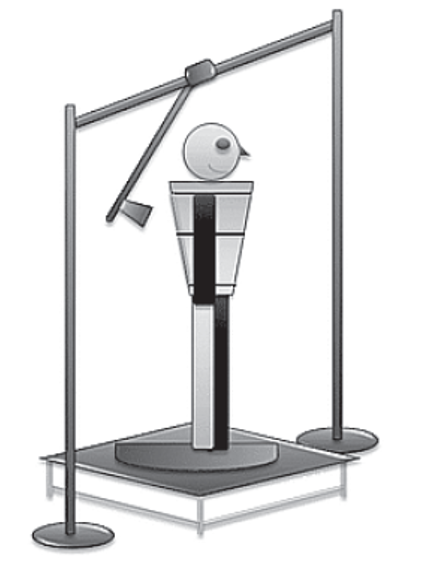
\includegraphics[width=1\linewidth]{images/human.png}
				\caption{Схематическое изображение толкателя
					и положения испытуемого на стабилоплатформе}
			\end{minipage}
			\hfill
			\begin{minipage}[h]{0.66\linewidth}
				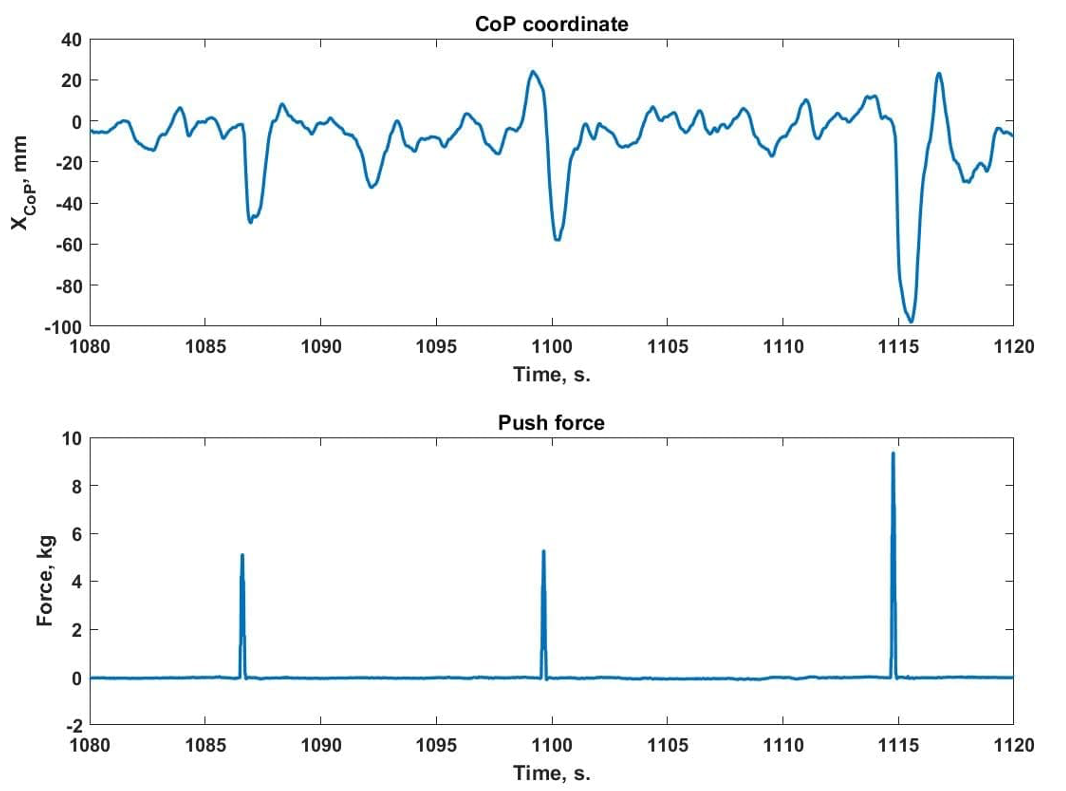
\includegraphics[width=1\linewidth]{images/Pushes.png}
				{\footnotesize
					\caption{Отклонение сагиттальной координаты при различных по силе толчках (данные предоставлены сотрудниками ИМБП РАН) }
				}
			\end{minipage}
		\end{center}
	\end{figure}
\end{frame}

\begin{frame}{Задача быстродействия}
	\begin{columns}
		\column{0.62\textwidth}
		\begin{figure}[h!]
			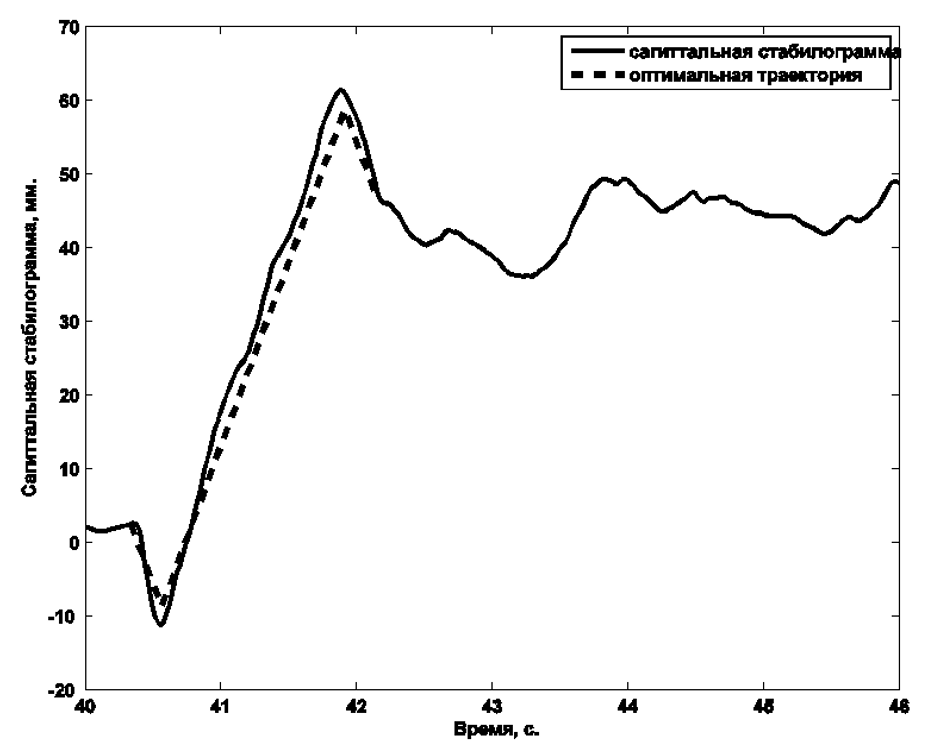
\includegraphics[width=1\linewidth]{images/stabilos.png}
			\caption{Характерный вид сагиттальной стабилограммы при выполнении теста со ступенчатым воздействием}
		\end{figure}
		\column{0.5\textwidth}
		% \column{\dimexpr\paperwidth-2pt}
		В работе рассматривается задача быстродействия для установки
		перевернутого маятника в неустойчивое вертикальное положение
		равновесия. Предполагается сравнение результатов стабилометрических
		проб, при которых человек возвращается в исходную вертикальную
		позу после толчка, с решением этой оптимальной задачи для начальных
		условий, соответствующих моменту времени завершения толчка.
	\end{columns}
\end{frame}

\begin{frame}{Математическая модель}
	\begin{columns}
		\column{0.62\textwidth}
		\begin{figure}[h!]
			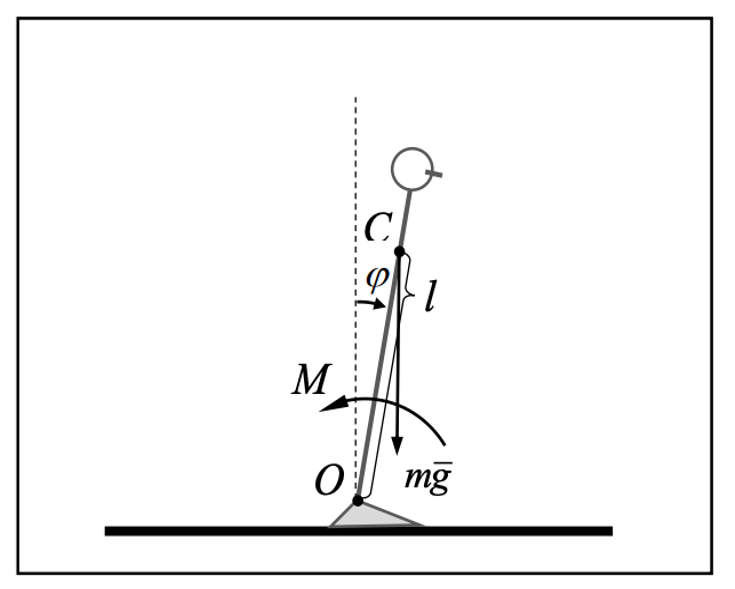
\includegraphics[width=1\linewidth]{images/inverse_pendulum.png}
			\caption{Модель перевернутого маятника}
		\end{figure}
		\column{0.5\textwidth}

		\[
			J\ddot{\varphi}=mgl\varphi+M
		\]
		\[
			\varphi(0)=\varphi_0; \dot{\varphi}(0)=\omega_0
		\]
		\[
			\varphi(t)=\varphi_k; \dot{\varphi}(t_k)=0
		\]
		\[
			M(0)=M(t_k)=-mgl\varphi_k
		\]
		\[
			U^-\leq\dot{M}\leq U^+
		\]
	\end{columns}
\end{frame}


\begin{frame}{Переход к безразмерным величинам}
	\[
		\theta^{''}=\theta+m;\ m^{'}=u
	\]
	\begin{columns}
		\column{0.3\textwidth}
		\[
			\theta=\frac{\varphi-\varphi_k}{\varphi_\ast},\ \ m=\frac{M-M_f}{mgl\varphi}
		\]
		\column{0.6\textwidth}
		Необходимо решение системы
		перевести из начального положения
		\[
			\theta(0)=1;\ \dot{\theta}(0)=\frac{t_\ast}{\varphi_\ast}\omega_0=\Omega_0;\ m(0)=0
		\]
		в положение
		\[
			\theta(\tau_f)=0;\ \dot{\theta}(\tau_f)=0;\ m(\tau_f)=0
		\]
		с помощью ограниченного управления
		\[
			u^-\le\ u\le\ u^+,\ \text{где } u^-=\frac{U^-}{mgl\varphi_\ast t_\ast}=-u^+
		\]

	\end{columns}
\end{frame}

\begin{frame}{Принцип максимума Понтрягина}
	Система в форме Коши
	\begin{equation}\label{koshisystem}
		\left\{ {\begin{aligned}
					 & \theta^{'} = \omega , \hfill   \\
					 & \omega^{'} = \theta+m , \hfill \\
					 & m^{'} = u . \hfill             \\
				\end{aligned}} \right.
	\end{equation}
	Функция Понтрягина
	\[
		H=\psi_1\cdot\omega+\psi_2\cdot(\theta+m)+\psi_3\cdot u
	\]

	Сопряженная система уравнений
	\begin{equation} \label{7}
		\left\{ {\begin{aligned}
					 & \dot \psi _1  = - \psi_1\hfill  \\
					 & \dot \psi _2   = - \psi_2\hfill \\
					 & \dot \psi _3   = - \psi_3 . \hfill        \\
				\end{aligned}} \right.
	\end{equation}

\end{frame}

\begin{frame}{Анализ сопряженной системы}
	\begin{equation}\label{psisystem}
		\left\{ {\begin{aligned}
					 & \psi_\theta = -C_1e^\tau+C_2e^{-\tau}+C_3, \hfill \\
					 & \psi_\omega = C_1e^\tau+C_2e^{-\tau} , \hfill     \\
					 & \psi_m = -C_1e^\tau+C_2e^{-\tau}+C_3 . \hfill     \\
				\end{aligned}} \right.
	\end{equation}
	Анализируя корни уравнения $\psi_3(\tau)=0$, для различной комбинации
	коэффициентов $C_1,C_2,C_3$, получим, что число корней не может быть больше двух. В системе может быть не более двух переключений $u$.
\end{frame}




\begin{frame}{Решение системы на 1 этапе}
	\begin{columns}
		\column{1\textwidth}
		Этап 1. $u=u_*$ начальные условия
		\[
			\theta(0)=1;\ \omega(0)=\Omega_0;\ m(0)=0
		\]
		Решение
		\begin{equation}\label{solvefull1stage}
			\left\{ {\begin{aligned}
						 & m_1(\tau) = u_*\tau, \hfill                                                                              \\
						 & \theta_1(\tau) = \frac{u_*+\Omega_0}{2}(e^\tau-e^{-\tau})+\frac{1}{2}(e^\tau+e^{-\tau})-u_*\tau , \hfill \\
						 & \omega_1(\tau) = \frac{1}{2}(e^\tau-e^{-\tau})+\frac{u_*+\Omega_0}{2}(e^\tau+e^{-\tau})-u_*  . \hfill    \\
					\end{aligned}} \right.
		\end{equation}
	\end{columns}
\end{frame}
\begin{frame}{Решение системы на 2 этапе}
	\begin{columns}
		\column{1\textwidth}
		Этап 2. $u=-u_*$ начальные условия
		\[
			\theta(\tau_1)=\theta_1(\tau_1);\ \omega(\tau_1)=\omega_1(\tau_1);\ m(\tau_1)=m_1(\tau_1)
		\]
		Решение
		{\footnotesize
		\begin{equation}\label{final2stage}
			\left\{ {\begin{aligned}
						 & m_2(\tau) = 2u_*\tau_1-u\tau, \hfill                                                                                                                            \\
						 & \theta_2(\tau) = \frac{u_*+\Omega_0}{2}(e^{\tau_1}-e^{-\tau_1})+\frac{1}{2}(e^{\tau_1}+e^{-\tau_1})-u_*(2\tau_1-e^{\tau_1-\tau}+e^{-\tau_1+\tau}-\tau) , \hfill \\
						 & \omega_2(\tau) = \frac{1}{2}(e^{\tau_1}-e^{-\tau_1})+\frac{u_*+\Omega_0}{2}(e^{\tau_1}+e^{-\tau_1})+u_*(1-e^{\tau_1-\tau}-e^{-\tau_1+\tau})  . \hfill           \\
					\end{aligned}} \right.
		\end{equation}
		}
	\end{columns}
\end{frame}
\begin{frame}{Решение системы на 3 этапе}
	\begin{columns}
		\column{1\textwidth}
		Этап 3. $u=u_*$ конечные условия
		\[
			\theta(\tau_f)=0;\ \omega(\tau_f)=0;\ m(\tau_f)=0
		\]
		Решение
		\begin{equation}\label{final3stage}
			\left\{ {\begin{aligned}
						 & m_3(\tau) = -u_*\tau_f+u_*\tau, \hfill                                                    \\
						 & \theta_3(\tau) = \frac{u_*}{2}(e^{-\tau_f+\tau}-e^{\tau_f-\tau})-u_*(\tau-\tau_f), \hfill \\
						 & \omega_3(\tau) = \frac{u_*}{2}(e^{-\tau_f+\tau}+e^{\tau_f-\tau})-u_*  . \hfill            \\
					\end{aligned}} \right.
		\end{equation}
	\end{columns}
\end{frame}

\begin{frame}{Сопряжение уравнений}
	\begin{equation}
		\left\{ {\begin{aligned}
					 & m_2(\tau_2) = m_3(\tau_2), \hfill            \\
					 & \theta_2(\tau_2) =  \theta_3(\tau_2), \hfill \\
					 & \omega_2(\tau_2) = \omega_3(\tau_2) . \hfill \\
				\end{aligned}} \right.
	\end{equation}
	\begin{columns}
		\column{1.2\textwidth}
		{\footnotesize
			\begin{equation}
				\footnotesize\left\{ {\begin{aligned}
							 & \tau_f=2(\tau_2-\tau_1), \hfill                                                                                                                                                                 \\
							 & \frac{u_*}{2}(e^{-\tau_f+\tau_2}-e^{\tau_f-\tau_2}) =\frac{u_*+\Omega_0}{2}(e^{\tau_1}-e^{-\tau_1})+\frac{1}{2}(e^{\tau_1}+e^{-\tau_1})-u_*(-e^{\tau_1-\tau_2}+e^{-\tau_1+\tau_2}), \hfill      \\
							 & \frac{u_*}{2}(e^{-\tau_f+\tau_2}+e^{\tau_f-\tau_2})-2u_*=\frac{1}{2}(e^{\tau_1}-e^{-\tau_1})+\frac{u_*+\Omega_0}{2}(e^{\tau_1}+e^{-\tau_1})+u_*(-e^{\tau_1-\tau_2}-e^{-\tau_1+\tau_2}) . \hfill \\
						\end{aligned}} \right.
			\end{equation}
		}
	\end{columns}
\end{frame}

\begin{frame}{Замена переменных}
	\[
		x=e^{\tau_1} ,\,\,y=e^{\tau_2} ,\,\,z=e^{\frac{\tau_f}{2}}
	\]
	\begin{equation}\label{findtau3}
		\left\{ {\begin{aligned}
					 & z=\frac{y}{x}, \hfill                                                                                                                                         \\
					 & \frac{u_*}{2}\big(\frac{y}{z^2}-\frac{z^2}{y}\big)=\frac{u_*+\Omega_0}{2}(x-\frac{1}{x})+\frac{1}{2}(x+\frac{1}{x})-u_*(\frac{y}{x}-\frac{x}{y}), \hfill      \\
					 & \frac{u_*}{2}\big(\frac{y}{z^2}+\frac{z^2}{y}\big)-2u_*=\frac{1}{2}(x-\frac{1}{x})+\frac{u_*+\Omega_0}{2}(x+\frac{1}{x})-u_*(\frac{y}{x}+\frac{x}{y}). \hfill \\
				\end{aligned}} \right.
	\end{equation}
\end{frame}



\begin{frame}{Заключение}


\end{frame}


\begin{frame}{Используемая литература}

	\begin{thebibliography}{3}
		\bibitem{Kim} Атанс М., Фалб П., Оптимальное управление. Москва, Машиностроение, 1968, 764 с.
		\bibitem{Pontryagin} Понтрягин Л.С., Болтянский В.Г., Гамкрелидзе Р.В., Мищенко Е.Ф. Математическая теория оптимальных процессов. Москва, Наука, 1983, 393 с.\\
		\bibitem{Most} Мостовской А.П. Численные методы и система Mathematica. Мурманск: 2009. - 249 с.
	\end{thebibliography}

\end{frame}


\end{document}